\documentclass[UTF8,a4paper,11pt,fontset=fandol]{ctexart}
\usepackage[margin=25mm,headheight=15pt]{geometry}
\usepackage{amsmath,amssymb,amsthm,mathtools,booktabs,array,graphicx}
\usepackage{enumitem,fancyhdr,xcolor,hyperref}
\usepackage{tikz}
\hypersetup{colorlinks=true,linkcolor=blue!40!black,citecolor=blue!40!black,urlcolor=blue!40!black,
pdftitle={三行矩形多米诺铺法的对称计数及奇数高度推广},
pdfauthor={本地研究稿，AI 辅助整理}}
\newtheorem{theorem}{定理}[section]
\newtheorem{lemma}[theorem]{引理}
\newtheorem{proposition}[theorem]{命题}
\newtheorem{corollary}[theorem]{推论}
\theoremstyle{definition}
\newtheorem{definition}[theorem]{定义}
\theoremstyle{remark}
\newtheorem{remark}[theorem]{注}
\renewcommand{\proofname}{证明}
\newcommand{\Fix}{\operatorname{Fix}}
\newcommand{\Stab}{\operatorname{Stab}}
\newcommand{\rev}{\operatorname{rev}}
\newcommand{\one}{\boldsymbol{1}}
\newcommand{\evec}{e_0}
\newcommand{\trans}{\mathsf T}
\numberwithin{equation}{section}
\setlength{\parskip}{0.3em}
\setlist{nosep}
\allowdisplaybreaks[2]
\pagestyle{fancy}
\fancyhf{}
\fancyhead[L]{\small 三行矩形多米诺铺法的对称计数}
\fancyhead[R]{\small 研究稿 v1.0}
\fancyfoot[C]{\thepage}
\title{\bfseries 三行矩形多米诺铺法的对称计数\\[4pt]
\large 基本块、半棋盘与奇数高度推广}
\author{本地研究稿}
\date{2026 年 10 月 25 日\quad 版本 1.0}
\begin{document}
\maketitle
\begin{abstract}
本文研究无标号多米诺对三行、偶数列矩形的全部铺法在旋转和反射下的轨道计数。
首先利用完整的列切口转移规则，将铺法唯一分解为不可竖切基本块，并把对称作用转化为字母对合和字的倒序。
由此给出 OEIS A232622 所列生成函数及七阶递推的完整推导。
其次建立半棋盘与对称固定铺法之间的双射，以两维递推重新得到三行公式，
并确定各精确稳定子类型及其渐近比例。
同一半棋盘方法给出任意固定奇数高度的轨道生成函数矩阵表达式及有理性；
五行情形进一步得到显式有理式、十四阶递推和六维多项式证书。
文中将一般证明、有限枚举与符号计算的作用分开，附可复现材料说明。
\end{abstract}
\noindent\textbf{关键词：} 多米诺铺法；Burnside 引理；生成函数；转移矩阵；对称轨道

\medskip
\noindent\textbf{稿件说明。}
本稿由本地 P002 研究记录整理，推导、代码及文字使用 Codex 辅助完成。
当前已作同一助手的书面自查与本地计算交叉核验，尚无独立外部审阅或形式化验证。
本文给出可逐步检查的证明，不作首次证明或文献优先权声明；作者署名由后续正式投稿时确定。

\section{问题、记号与主要结果}
\label{sec:intro}

\subsection{计数对象与文献背景}
对整数 $n\ge1$，令 $\mathcal T_n$ 为 $3\times2n$ 单位格矩形的全部多米诺铺法。
每块砖覆盖两个共边相邻的格子，允许横放或竖放；铺法是这些无序格对的集合，
砖不带标号，不重叠、不留空，也不施加 tatami 条件。
行号从上到下为 $r=1,2,3$，列号从左到右为 $c=1,\ldots,2n$。定义
\[
 h(r,c)=(4-r,c),\qquad v(r,c)=(r,2n+1-c),\qquad \rho=hv.
\]
记 $G=\{e,h,v,\rho\}$，其中 $h$ 为上下反射，$v$ 为左右反射，$\rho$ 为半周旋转。
因为 $3\ne2n$，$G$ 是保持该矩形的完整平面等距对称群。
令 $a(n)=|\mathcal T_n/G|$。对 $n=0$，规定只有一个空铺法，四个抽象群元素均固定它，
故 $a(0)=1$。此约定允许群作用不忠实。

Mathar \cite{mathar2013} 的表 10 和 Conjecture 6 给出三行对称轨道计数及其猜想生成函数；
OEIS A232622 \cite{oeis} 列有等价的有理式和七阶递推。
截至 2026 年 10 月 25 日，本地核查的 OEIS 页面仍保留猜想标签。
这说明该页面的表述状态，不足以说明全部文献中仍无证明。
本文的目标是给出这组公式的自足推导，并整理其对称细化与奇数高度推广。

固定宽度铺法的有限状态方法是已有工具。Mathar \cite{mathar2014} 的第 2.1--2.3 节
讨论了三行普通铺法和不可竖切块的生成函数。
本文重新证明所需块分类，补充反射和旋转在基本块字上的作用，
并用另一种半棋盘双射处理固定点。本文不以文献中的目标猜想、
有限数列或程序输出作为一般证明的前提。

\subsection{主定理}
四类固定点数分别记为
\[
 d_n=|\mathcal T_n|,\quad h_n=|\Fix(h)|,\quad
 v_n=|\Fix(v)|,\quad r_n=|\Fix(\rho)|,
\]
其以半长度 $n$ 为指数的普通生成函数记为 $D,H,V,R$。
除渐近分析外，本文所有生成函数都在 $\mathbb Q[[x]]$ 中解释。

\begin{theorem}[三行对称轨道的生成函数]\label{thm:main}
对上述全部铺法，有
\begin{equation}\label{eq:main}
 A(x):=\sum_{n\ge0}a(n)x^n
 =\frac{1-3x-4x^2+10x^3-4x^5+x^6}
 {(1-x)(1-4x+x^2)(1-4x^2+x^4)}.
\end{equation}
相应递推为
\begin{equation}\label{eq:recurrence}
\begin{split}
a(n)={}&5a(n-1)-a(n-2)-19a(n-3)+19a(n-4)\\
       &+a(n-5)-5a(n-6)+a(n-7),\qquad n\ge7,
\end{split}
\end{equation}
初值为 $(a(0),\ldots,a(6))=(1,2,5,14,46,156,561)$。
\end{theorem}

式 \eqref{eq:main} 分子、分母同乘 $-1$ 即得到 OEIS 所列形式。
第 \ref{sec:blocks} 节给出基本块证明；
第 \ref{sec:half} 节用半棋盘方法重新推导四类固定点数。
第 \ref{sec:types} 节确定精确稳定子并研究对称比例；
第 \ref{sec:odd} 节推广到任意固定奇数高度，
第 \ref{sec:five} 节给出五行显式实例。五行计算所需的全部小矩阵在附录中列出。

\begin{lemma}[轨道平均公式]\label{lem:burnside}
对每个 $n\ge0$，
\begin{equation}\label{eq:burnside}
 a(n)=\frac{d_n+h_n+v_n+r_n}{4}.
\end{equation}
\end{lemma}
\begin{proof}
双重计数集合 $\{(g,T):g\in G,\ T\in\mathcal T_n,\ gT=T\}$ 得
\[
 \sum_{g\in G}|\Fix(g)|=\sum_{T\in\mathcal T_n}|\Stab(T)|.
\]
轨道稳定子公式表明，一个轨道 $O$ 对右边的贡献为
$|O|\cdot4/|O|=4$，故得所需等式。
这也是 Burnside 引理 \cite[第 7 章，Lemma 7.2]{stanley} 在本问题的应用。
上述计数不要求作用忠实，因而包含空棋盘。
\end{proof}

\section{基本块分解与第一种证明}\label{sec:blocks}

\subsection{列切口的完整状态规则}
先考虑任意宽度 $w$ 的三行棋盘。在第 $j$ 列与第 $j+1$ 列之间记
$S_j\subseteq\{1,2,3\}$ 为被水平砖跨越的行集合，端点取
$S_0=S_w=\varnothing$。
若一列的输入和输出状态分别为 $p,q$，则合法的充要条件为
\begin{equation}\label{eq:local3}
 p\cap q=\varnothing,\qquad
 \{1,2,3\}\setminus(p\cup q)\in
 \{\varnothing,\{1,2\},\{2,3\}\}.
\end{equation}
理由是输入行的格已被左来的砖占用，输出行用于向右的砖，其余格必须在本列用竖直砖配对。
每个合法转移的本列填充唯一。全部转移见表 \ref{tab:states}。

\begin{table}[htbp]
\centering
\caption{三行的完整列状态转移。}\label{tab:states}
\begin{tabular}{cc@{\qquad}cc}
\toprule
输入 & 全部输出 & 输入 & 全部输出\\
\midrule
$\varnothing$ & $\{1\},\{3\},\{1,2,3\}$ &
$\{1,2\}$ & $\{3\}$\\
$\{1\}$ & $\varnothing,\{2,3\}$ &
$\{1,3\}$ & $\{2\}$\\
$\{2\}$ & $\{1,3\}$ &
$\{2,3\}$ & $\{1\}$\\
$\{3\}$ & $\varnothing,\{1,2\}$ &
$\{1,2,3\}$ & $\varnothing$\\
\bottomrule
\end{tabular}
\end{table}

\begin{lemma}\label{lem:path}
三行、$w$ 列的完整铺法与表 \ref{tab:states} 中长度为 $w$、
从空状态回到空状态的合法路径一一对应。
\end{lemma}
\begin{proof}
铺法唯一确定各切口状态。反过来，在每个切口状态指定的行放跨切口水平砖，
再在每列剩余行放唯一的竖直砖。式 \eqref{eq:local3} 保证同格不被两个水平砖重复使用，
且剩余格恰好被竖直砖覆盖。端点空状态排除越界砖。
两种构造互逆；$w=0$ 对应空路径。
\end{proof}

\subsection{首次回返路径与不可竖切块}
\begin{definition}
若一个内部竖直格线没有砖跨越，称它为断口。
非空完整铺法若没有内部断口，称为基本块。
\end{definition}

\begin{lemma}[基本块分类]\label{lem:blocks}
所有三行基本块恰为 $C$ 及 $A_k,B_k$（$k\ge1$）。
其中 $C$ 为宽 2 的三块水平砖；$A_k$ 宽 $2k$，由下列砖组成：
\begin{enumerate}
\item 第 1 列和第 $2k$ 列各放一块覆盖第 1、2 行的竖直砖；
\item 第 3 行按列对 $(2j-1,2j)$ 铺满，$1\le j\le k$；
\item 第 1、2 行内部各按列对 $(2j,2j+1)$ 铺满，$1\le j<k$。
\end{enumerate}
最后令 $B_k=h(A_k)$。
\end{lemma}
\begin{proof}
基本块对应空状态的首次回返路径。从空状态出发只有三个分支。
若第一步到 $\{1,2,3\}$，下一步被迫回空状态，给出 $C$。
若第一步到 $\{3\}$，则在最终回空状态之前，
只能在 $\{3\}$ 与 $\{1,2\}$ 之间交替。路径恰为
\[
 \varnothing\longrightarrow\{3\}
 \longrightarrow
 \bigl(\{1,2\}\longrightarrow\{3\}\bigr)^{k-1}
 \longrightarrow\varnothing,\qquad k\ge1,
\]
这里括号内表示两步的重复，$k=1$ 时重复零次。
路径给出所述 $A_k$ 坐标。第一步到 $\{1\}$ 的分支
只能在 $\{1\},\{2,3\}$ 之间交替后回空状态，得到 $B_k$。
表 \ref{tab:states} 穷尽了这些分支的所有后继，因而无遗漏。
$A_k$ 的奇数内部切口由第 3 行水平砖跨越，
偶数内部切口由第 1、2 行水平砖跨越，故确实无断口；
$B_k$ 由反射得到同样性质。
首列的竖直砖位置区分 $A_k,B_k$，而 $C$ 无竖直砖，故无重计。
\end{proof}

\begin{figure}[htbp]
\centering
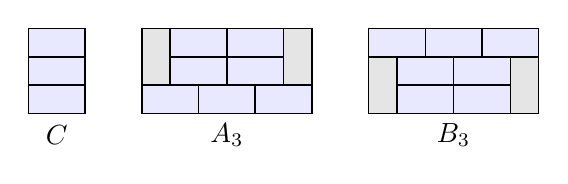
\begin{tikzpicture}[x=0.36cm,y=0.36cm,line width=0.55pt]
\begin{scope}
 \foreach \y in {0,1,2}{\draw[fill=blue!9] (0,\y) rectangle ++(2,1);}
 \node at (1,-0.75) {$C$};
\end{scope}
\begin{scope}[shift={(4,0)}]
 \draw[fill=gray!20] (0,1) rectangle (1,3);
 \draw[fill=gray!20] (5,1) rectangle (6,3);
 \foreach \x in {0,2,4}{\draw[fill=blue!9] (\x,0) rectangle ++(2,1);}
 \foreach \y in {1,2}{\foreach \x in {1,3}{\draw[fill=blue!9] (\x,\y) rectangle ++(2,1);}}
 \node at (3,-0.75) {$A_3$};
\end{scope}
\begin{scope}[shift={(12,0)}]
 \draw[fill=gray!20] (0,0) rectangle (1,2);
 \draw[fill=gray!20] (5,0) rectangle (6,2);
 \foreach \x in {0,2,4}{\draw[fill=blue!9] (\x,2) rectangle ++(2,1);}
 \foreach \y in {0,1}{\foreach \x in {1,3}{\draw[fill=blue!9] (\x,\y) rectangle ++(2,1);}}
 \node at (3,-0.75) {$B_3$};
\end{scope}
\end{tikzpicture}

\caption{三种基本块的代表 $C,A_3,B_3$。矩形边界表示实际砖界；图示不代替一般分类证明。}
\label{fig:blocks}
\end{figure}

\begin{lemma}[唯一块分解及对称作用]\label{lem:word}
每个完整三行铺法唯一对应基本块字母表
$\mathcal B=\{C\}\cup\{A_k,B_k:k\ge1\}$ 上的一个有限字。
令 $\sigma$ 固定 $C$，交换 $A_k$ 与 $B_k$，则字上的作用为
\begin{equation}\label{eq:word-action}
 h(W)=\sigma(W),\qquad v(W)=\rev(W),\qquad
 \rho(W)=\sigma(\rev(W)).
\end{equation}
\end{lemma}
\begin{proof}
沿全部断口切开，所得各段无内部断口，故由引理 \ref{lem:blocks} 都是基本块。
任何基本块分解的分界必须是断口，而且不能遗漏断口，
否则有一块内部仍可竖切。这证明唯一性。任意基本块字的拼接给出逆映射。

上下反射在各块内按定义施加 $\sigma$。每个基本块还都左右对称：
对 $A_k$，列反转 $c\mapsto2k+1-c$ 交换两端竖直砖，
将底行列对 $(2j-1,2j)$ 映为同类列对，
将上两行列对 $(2j,2j+1)$ 映为同类列对；
对应指标分别为 $k+1-j$ 和 $k-j$。$C$ 逐砖不变。
由于上下、左右反射交换，$B_k=h(A_k)$ 也左右对称。

全棋盘反射保持断口集合；上下反射保留块次序，
左右反射颠倒块次序。结合唯一分解即得 \eqref{eq:word-action}。
论证允许相邻块宽度不同。
\end{proof}

\subsection{固定字的生成函数}
给 $C$ 权 $x$，给 $A_k,B_k$ 权 $x^k$，权的指数为半长度。
基本块生成函数为
\begin{equation}\label{eq:F}
 F(x)=x+2\sum_{k\ge1}x^k=\frac{3x-x^2}{1-x}.
\end{equation}
由于 $F(0)=0$，每个次数只涉及有限多个字，形式求和合法。

\begin{proposition}\label{prop:fixed-gf}
四种固定点生成函数为
\begin{align}
D(x)&=\frac{1}{1-F(x)}=\frac{1-x}{1-4x+x^2},&
H(x)&=\frac{1}{1-x},\label{eq:DH}\\
V(x)&=(1+F(x))D(x^2)
 =\frac{1+3x+x^2-x^3}{1-4x^2+x^4},\label{eq:V}\\
R(x)&=(1+x)D(x^2)
 =\frac{1+x-x^2-x^3}{1-4x^2+x^4}.\label{eq:R}
\end{align}
\end{proposition}
\begin{proof}
普通铺法对应任意字，故 $D=\sum_{\ell\ge0}F^\ell$。
上下反射固定字的每个字母须由 $\sigma$ 固定，唯一选择为 $C$，
故 $H=\sum_{\ell\ge0}x^\ell$。

左右反射固定字是回文，唯一写为
$U\rev(U)$ 或 $Ub\rev(U)$，其中 $b$ 为任意基本块。
两侧的总权是左侧权的平方，所以左半字贡献 $D(x^2)$，
中间贡献 $1+F(x)$，得到 \eqref{eq:V}。

半周旋转固定字唯一写为
$U\sigma(\rev(U))$，或 $Ub\sigma(\rev(U))$ 且 $\sigma(b)=b$。
后一种情形只允许 $b=C$，故中心贡献 $1+x$。
这两类互斥，分解可逆，得到 \eqref{eq:R}。
中心基本块允许跨越几何中线；上述计数没有附加中线必须为断口的限制。
\end{proof}

\begin{proof}[定理 \ref{thm:main} 的第一种证明]
由引理 \ref{lem:burnside} 和命题 \ref{prop:fixed-gf}，
\begin{equation}\label{eq:average-rational}
 A(x)=\frac14\left[
 \frac{1-x}{1-4x+x^2}+\frac1{1-x}
 +\frac{2(1+2x-x^3)}{1-4x^2+x^4}\right].
\end{equation}
记 $P_3=1-4x+x^2$、$Q_3=1-4x^2+x^4$。
通分后分子为
\[
 \frac{(1-x)^2Q_3+P_3Q_3+
 2(1+2x-x^3)(1-x)P_3}{4}
 =1-3x-4x^2+10x^3-4x^5+x^6.
\]
这给出 \eqref{eq:main}。分母展开为
\[
 1-5x+x^2+19x^3-19x^4-x^5+5x^6-x^7.
\]
因分子次数为 6，比较次数 $n\ge7$ 的系数得到
\eqref{eq:recurrence}；比较次数 $0,\ldots,6$ 得到所述初值。
\end{proof}

Mathar \cite[式 (26)]{mathar2013} 以全列数为指数，故与本文比较应取
$\overline T(z,3)=A(z^2)$。将 $x=z^2$ 代入
\eqref{eq:average-rational}，第一项重排利用
$\tfrac18((1+z)^{-1}+(1-z)^{-1})=(4(1-z^2))^{-1}$，
即得到该文献的表达式。
Mathar \cite[式 (4)--(6)]{mathar2014} 的三行公式以砖数计次，
对应换元为 $z^3=x$。两种变量约定不可混用。

\section{半棋盘双射与第二种证明}\label{sec:half}
本节从局部覆盖重新构造计数，不使用基本块分类或回文公式。
为便于后续推广，先允许任意整数高度 $m\ge1$。

\subsection{带末端半块的部分铺法}
对 $j\ge1$ 和 $S\subseteq\{1,\ldots,m\}$，令 $\mathcal P_m(j,S)$ 为
$m\times j$ 棋盘的部分铺法：除末列行号属于 $S$ 的格外，所有格都由内部多米诺覆盖；
这些未覆盖格标记为向右伸出的半块，准备与右邻格配成水平砖。
$j=0$ 时只有 $S=\varnothing$ 的空对象。记 $q_j(S)=|\mathcal P_m(j,S)|$。

令 $T_m$ 的行列按所有行子集排列。定义
\begin{equation}\label{eq:Tm}
 T_m[p,q]=
 \begin{cases}
 1,&p\cap q=\varnothing,\text{ 且 }[m]\setminus(p\cup q)
       \text{ 的每个连续段均为偶长},\\
 0,&\text{否则}.
 \end{cases}
\end{equation}
这里 $[m]=\{1,\ldots,m\}$，空补集满足条件。
每段偶长剩余行的竖直配对唯一，因为端点只能与相邻格配对，
剥去此对后继续。奇长段无法配满。
因此 \eqref{eq:Tm} 恰好刻画加一列的合法转移。
放入指定水平砖和唯一竖直配对给出逆构造，故
\begin{equation}\label{eq:profile}
 q_j^{\trans}=\evec^{\trans}T_m^j,\qquad
 t_m(j)=\evec^{\trans}T_m^j\evec,
\end{equation}
其中 $\evec$ 是空状态的单位列向量，$t_m(j)$ 为完整 $m\times j$ 铺法数。
辅助定义 $T_0=(1)$、$t_0(j)=1$。

\subsection{对称固定铺法的边界条件}
记 $J(S)=\{m+1-r:r\in S\}$，$\one$ 为全 1 列向量，
$\chi_m(S)=1$ 当且仅当 $J(S)=S$。
用 $v_{m,n},r_{m,n}$ 表示 $m\times2n$ 的左右反射、半周旋转固定数。

\begin{lemma}[中线补全双射]\label{lem:half}
对 $m\ge1$ 和 $n\ge0$，
\begin{equation}\label{eq:half-fixed}
 v_{m,n}=\evec^{\trans}T_m^n\one,\qquad
 r_{m,n}=\evec^{\trans}T_m^n\chi_m.
\end{equation}
\end{lemma}
\begin{proof}
先设 $n\ge1$。任取 $P\in\mathcal P_m(n,S)$，
将内部砖左右反射到右半棋盘，然后对每个 $r\in S$
插入连接 $(r,n)$ 与 $(r,n+1)$ 的水平砖。
两半内部砖不相交，跨中线砖恰好补齐剩余格，
得到唯一的左右反射固定铺法。
反向限制到左半，切断跨中线砖，唯一恢复 $P,S$，
因此所有 $S$ 都可取，并有第一式。

对半周旋转，将左半内部砖旋转到右半后，右侧待补行集合为 $J(S)$。
跨中线砖必须水平，故能补全的充要条件是 $J(S)=S$。
条件满足时逐行插入跨中线砖，所得砖集合在半周旋转下保持不变；
限制到左半是逆操作，得到第二式。
条件的必要性也来自跨中线第 $r$ 行的砖必须有第 $m+1-r$ 行的旋转像。
$n=0$ 时只有空对象，两式均为 1。
\end{proof}

\begin{lemma}[奇数高度的上下反射]\label{lem:h-odd}
若 $m=2k+1$，$k\ge0$，则
\begin{equation}\label{eq:h-odd}
 h_{m,n}=t_k(2n).
\end{equation}
\end{lemma}
\begin{proof}
在上下反射固定铺法中，接触中央行的竖直砖会被映到另一块竖直砖，
两者在中央行重叠，因此不存在这样的砖。
中央行只能以唯一方式水平铺满。其上 $k$ 行必须自行铺满，
下方由其反射唯一确定。任意上方完整铺法都给出一个固定铺法，
限制回上方为逆操作。$k=0$ 与 $n=0$ 由空对象约定覆盖。
\end{proof}

\subsection{三行的两维递推}
对 $m=3$，由 \eqref{eq:Tm} 从空状态可达的状态恰为
$\varnothing,\{1\},\{3\},\{1,2\},\{2,3\},\{1,2,3\}$。
规则给出空集的输出为两个端点单集和全体集合；
$\{1\}$ 的输出为 $\varnothing,\{2,3\}$，
$\{3\}$ 的输出为 $\varnothing,\{1,2\}$，
其余三个状态的输出分别被迫为 $\{3\},\{1\},\varnothing$。
从初始计数归纳可得
\[
 q_{2j}(\varnothing)=\alpha_j,\qquad
 q_{2j}(\{1,2\})=q_{2j}(\{2,3\})=\beta_j;
\]
一步后仅有
\[
 q_{2j+1}(\{1\})=q_{2j+1}(\{3\})=\alpha_j+\beta_j,\qquad
 q_{2j+1}(\{1,2,3\})=\alpha_j.
\]
再次转移于是得到
\begin{equation}\label{eq:two-dimensional}
 \binom{\alpha_{j+1}}{\beta_{j+1}}
 =\begin{pmatrix}3&2\\1&1\end{pmatrix}
 \binom{\alpha_j}{\beta_j},\qquad
 (\alpha_0,\beta_0)=(1,0).
\end{equation}
这同时证明了所列非零状态的归纳封闭性。

\begin{proposition}\label{prop:parity}
设 $d_j=t_3(2j)$，则
\begin{equation}\label{eq:d-rec}
 d_0=1,\quad d_1=3,\quad d_{j+2}=4d_{j+1}-d_j\quad(j\ge0).
\end{equation}
三行固定点数满足
\begin{equation}\label{eq:parity-fixed}
 h_n=1,\quad r_{2j}=r_{2j+1}=d_j,\quad
 v_{2j}=d_{j+1}-2d_j,\quad v_{2j+1}=d_{j+1}.
\end{equation}
因此
\begin{equation}\label{eq:parity-orbits}
 a(2j)=\frac{d_{2j}+1+d_{j+1}-d_j}{4},\qquad
 a(2j+1)=\frac{d_{2j+1}+1+d_{j+1}+d_j}{4}.
\end{equation}
\end{proposition}
\begin{proof}
由 \eqref{eq:profile}，$d_j=\alpha_j$。
式 \eqref{eq:two-dimensional} 中的矩阵满足 $M^2-4M+I=0$，
从而得 \eqref{eq:d-rec}。
偶数步可达的 $J$-不变集合只有空集，
奇数步可达的 $J$-不变集合只有全三行集合，故引理 \ref{lem:half} 给出 $r$ 的两式。
对所有状态求和，偶数步得
$\alpha_j+2\beta_j=d_{j+1}-2d_j$，
奇数步得 $3\alpha_j+2\beta_j=d_{j+1}$。
引理 \ref{lem:h-odd} 给出 $h_n=t_1(2n)=1$。
最后代入轨道平均公式即得 \eqref{eq:parity-orbits}。
\end{proof}

\begin{proof}[定理 \ref{thm:main} 的第二种证明]
递推 \eqref{eq:d-rec} 给出 $D(x)=(1-x)/(1-4x+x^2)$。
对 \eqref{eq:parity-fixed} 分别求和可得
\[
 H(x)=\frac1{1-x},\quad R(x)=(1+x)D(x^2),\quad
 V(x)=(1+x)\frac{D(x^2)-1}{x^2}-2D(x^2).
\]
因 $D(t)-1$ 的常数项为零，除以 $t$ 在形式幂级数中合法。
化简 $V$ 得到 \eqref{eq:V}，再用轨道平均公式即得
\eqref{eq:average-rational}，其通分和系数比较已在前文完整写出。
本次推导的组合前提仅为半棋盘双射和单列覆盖规则。
\end{proof}

\section{精确对称类型与渐近行为}\label{sec:types}

\begin{theorem}[精确稳定子分类]\label{thm:stabilizers}
对三行、$2n$ 列棋盘，各精确稳定子的铺法数和轨道数见表 \ref{tab:stabilizers}。
该表对所有 $n\ge0$ 成立。
\end{theorem}
\begin{table}[htbp]
\centering
\caption{三行铺法的全部精确稳定子类型。}\label{tab:stabilizers}
\begin{tabular}{cccc}
\toprule
精确稳定子 & 铺法数 & 轨道大小 & 轨道数\\
\midrule
$G$ & $1$ & $1$ & $1$\\
$\{e,h\}$ & $0$ & $2$ & $0$\\
$\{e,v\}$ & $v_n-1$ & $2$ & $(v_n-1)/2$\\
$\{e,\rho\}$ & $r_n-1$ & $2$ & $(r_n-1)/2$\\
$\{e\}$ & $d_n-v_n-r_n+1$ & $4$ & $(d_n-v_n-r_n+1)/4$\\
\bottomrule
\end{tabular}
\end{table}
\begin{proof}
引理 \ref{lem:h-odd} 表明唯一的上下反射固定铺法是三行各自水平铺满的铺法，
它同时被 $v,\rho$ 固定。
若铺法同时由任意两个不同的非恒等群元素固定，则也由它们的积固定，
因而由整个 $G$ 固定。故三种固定集的两两交集和三重交集都是上述单点。
于是只具 $v$ 对称的铺法有 $v_n-1$ 个，只具 $\rho$ 对称的有 $r_n-1$ 个，
只具 $h$ 对称的有零个；其余 $d_n-v_n-r_n+1$ 个的稳定子平凡。
群 $G$ 交换，同一轨道中的稳定子相同。各类除以轨道大小即得表中结果。
四元群的子群只有表中五种，故分类完整。
\end{proof}

例如 $n=8$ 时 $d_8=29681,v_8=265,r_8=153$。
共有 $7525$ 个轨道，其中 $7316$ 个稳定子平凡，
$132$ 个精确稳定子为 $\{e,v\}$，$76$ 个为 $\{e,\rho\}$，$1$ 个为 $G$。

\begin{theorem}[对称铺法的渐近比例]\label{thm:asym}
令 $\lambda=2+\sqrt3$。均匀选取一个有固定棋盘方向的普通铺法时，
其具有非平凡对称的概率 $p_n$ 满足
\begin{align}
 p_{2j}&\sim(\lambda-1)\lambda^{-j},&
 p_{2j+1}&\sim\frac{\lambda+1}{\lambda}\lambda^{-j}
 \quad(j\to\infty).\label{eq:prob-asym}
\end{align}
特别地，$p_n=O(\lambda^{-n/2})\to0$，并且
\begin{equation}\label{eq:orbit-asym}
 a(n)=\frac{d_n}{4}+O(\lambda^{n/2})
 \sim\frac{3+\sqrt3}{24}\lambda^n.
\end{equation}
\end{theorem}
\begin{proof}
由 \eqref{eq:d-rec} 的特征根和初值，
\begin{equation}\label{eq:d-closed}
 d_n=c_+\lambda^n+c_-\lambda^{-n},\qquad
 c_+=\frac{3+\sqrt3}{6},\quad c_-=\frac{3-\sqrt3}{6}.
\end{equation}
表 \ref{tab:stabilizers} 给出
$p_n=(v_n+r_n-1)/d_n$。
而 \eqref{eq:parity-fixed} 给出
\[
 v_{2j}+r_{2j}=d_{j+1}-d_j,\qquad
 v_{2j+1}+r_{2j+1}=d_{j+1}+d_j.
\]
将 \eqref{eq:d-closed} 代入，分子主项分别为
$c_+(\lambda-1)\lambda^j$ 与 $c_+(\lambda+1)\lambda^j$，
分母主项分别为 $c_+\lambda^{2j}$ 与 $c_+\lambda^{2j+1}$，
故得 \eqref{eq:prob-asym}。
最后由 $a(n)=(d_n+1+v_n+r_n)/4$ 得到 \eqref{eq:orbit-asym}。
\end{proof}

如果均匀选取的是轨道，则非平凡对称轨道数为
$1+(v_n-1)/2+(r_n-1)/2=(v_n+r_n)/2$，
其比例为 $(v_n+r_n)/(2a(n))$，同样趋于零，但这是不同的概率空间。

\section{任意固定奇数高度的矩阵公式}\label{sec:odd}

现在固定 $m=2k+1\ge1$，以 $a_m(n)$ 记全部 $m\times2n$ 多米诺铺法
在完整矩形对称群下的轨道数，空棋盘计 1。
正高度为奇数，正宽度为偶数，非空棋盘不可能为正方形，
因此仍使用四元群 $\{e,h,v,\rho\}$。
矩阵 $T_m$、行反转指标 $\chi_m$ 及边界向量采用第 \ref{sec:half} 节的定义。

\begin{theorem}[奇数高度的轨道公式]\label{thm:odd}
对每个固定 $m=2k+1\ge1$ 和全部 $n\ge0$，
\begin{equation}\label{eq:odd-count}
 a_m(n)=\frac14\left[
 \evec^{\trans}T_m^{2n}\evec
 +\evec^{\trans}T_k^{2n}\evec
 +\evec^{\trans}T_m^n(\one+\chi_m)\right].
\end{equation}
其生成函数为
\begin{equation}\label{eq:odd-gf}
\begin{split}
 A_m(x)=\frac14\bigl[&
 \evec^{\trans}(I-xT_m^2)^{-1}\evec
 +\evec^{\trans}(I-xT_k^2)^{-1}\evec\\
 &+\evec^{\trans}(I-xT_m)^{-1}(\one+\chi_m)\bigr].
\end{split}
\end{equation}
因而每个固定奇数高度的轨道生成函数都是有理函数，
计数序列满足某个常系数线性递推。
\end{theorem}
\begin{proof}
式 \eqref{eq:profile} 给出恒等项，
引理 \ref{lem:h-odd} 给出上下反射项，
引理 \ref{lem:half} 给出左右反射及半周旋转项。
对四元群应用引理 \ref{lem:burnside} 的同一双重计数论证，
即得 \eqref{eq:odd-count}。
对 $n$ 作形式求和，利用
$\sum_{n\ge0}x^n M^n=(I-xM)^{-1}$ 得 \eqref{eq:odd-gf}。
各矩阵有限，$I-xM$ 的常数项为单位矩阵，
故其逆存在；由伴随矩阵公式，每个元素都是有理函数。
有理生成函数乘以其常数项非零的分母，再比较充分高次数的系数，
得到常系数线性递推。
\end{proof}

各项的 $\evec$ 按对应矩阵空间解释，特别是 $k=0$ 时使用 $T_0=(1)$。
该定理的固定点边界向量已经明确给出，故可直接求任意指定奇数高度的精确表达式。
引理 \ref{lem:half} 本身允许偶数高度，
但上下反射式 \eqref{eq:h-odd} 依赖中央行。
偶数高度需要另行处理中轴上的竖直砖；
正方形若按全部对称取商，还必须加入四分之一周旋转和对角反射。
这些情形不包含在定理 \ref{thm:odd} 中。

\section{五行棋盘的显式生成函数}\label{sec:five}
五行情形可以把一般矩阵公式压缩为六维多项式恒等式。
为使此实例可手工复核，本节给出证书和全部边界向量，
附录 \ref{app:certificate} 列出单列转移的构造。

用五位掩码表示行集合，最低位对应顶行。
偶数列可达状态的行反转轨道依次为
\begin{equation}\label{eq:even-orbits}
 \{0\},\{3,24\},\{6,12\},\{9,18\},\{15,30\},\{27\}.
\end{equation}
计数在行反转下相同。令 $u_j$ 的六个分量表示第 $2j$ 列后
相应轨道中\emph{每个单独状态}的计数，非轨道计数之和。
则 $u_0=\evec$，$u_{j+1}=Mu_j$，其中
\begin{equation}\label{eq:M5}
 M=\begin{pmatrix}
8&6&4&2&2&1\\
3&4&1&1&1&1\\
2&1&2&1&1&0\\
1&1&1&2&1&0\\
1&1&1&1&1&0\\
1&2&0&0&0&1
\end{pmatrix}.
\end{equation}
设
\begin{equation}\label{eq:PN}
\begin{split}
 P(t)&=1-15t+32t^2-15t^3+t^4,\\
 N(t)&=\bigl(1-7t+7t^2-t^3,\ 
 3t-4t^2+t^3,\ 2t-5t^2+t^3,\ t+t^2,\ t-t^3,\ t-t^3\bigr)^{\trans}.
\end{split}
\end{equation}
直接多项式乘法给出
\begin{equation}\label{eq:certificate}
 (I-tM)N(t)=P(t)\evec.
\end{equation}
由于 $P(0)=1$，该恒等式证明
\[
 f(t):=\sum_{j\ge0}u_jt^j=\frac{N(t)}{P(t)}.
\]
附录还把式 \eqref{eq:certificate} 写成四个系数向量等式，
因此不需要将符号软件输出作为黑箱。

左右反射在偶数、奇数半长度的终端行向量分别为
\begin{align*}
 w_{v,e}&=(1,2,2,2,2,1),&w_{v,o}&=(8,6,4,4,2,1),
\end{align*}
半周旋转相应为
\[
 w_{r,e}=(1,0,0,0,0,1),\qquad w_{r,o}=(2,2,0,0,0,1).
\]
偶数终端向量分别累计所有状态，或仅累计行反转固定状态；
奇数终端向量先作一次单列转移再累计。
引理 \ref{lem:half} 因而给出
\begin{equation}\label{eq:terminal5}
 V_5(x)=(w_{v,e}+xw_{v,o})f(x^2),\qquad
 R_5(x)=(w_{r,e}+xw_{r,o})f(x^2).
\end{equation}

\begin{theorem}[五行显式公式]\label{thm:five}
令 $D_5,H_5,V_5,R_5$ 分别为五行四种固定点数的生成函数，则
\begin{align}
 D_5(x)&=\frac{1-7x+7x^2-x^3}{P(x)},&
 H_5(x)&=\frac{1-x}{1-3x+x^2},\label{eq:five-DH}\\
 V_5(x)&=\frac{1+8x+8x^2-23x^3-9x^4+16x^5-x^7}{P(x^2)},\label{eq:five-V}\\
 R_5(x)&=\frac{1+2x-6x^2-7x^3+7x^4+6x^5-2x^6-x^7}{P(x^2)}.\label{eq:five-R}
\end{align}
轨道生成函数为
\begin{equation}\label{eq:five-A}
 A_5(x)=\frac{D_5(x)+H_5(x)+V_5(x)+R_5(x)}4.
\end{equation}
\end{theorem}
\begin{proof}
普通完整铺法对应空终端状态，故 $D_5=f_0$，
给出 \eqref{eq:five-DH} 的第一式。
将 \eqref{eq:PN} 代入 \eqref{eq:terminal5} 给出
\eqref{eq:five-V} 和 \eqref{eq:five-R}。
由引理 \ref{lem:h-odd}，$h_{5,n}=t_2(2n)$。
两行铺法从最左列分类，或者首列由一块竖直砖覆盖，
或者前两列由两块水平砖覆盖，所以
$t_2(j)=t_2(j-1)+t_2(j-2)$，初值为 $t_2(0)=t_2(1)=1$。
其两步转移矩阵为
$\left(\begin{smallmatrix}2&1\\1&1\end{smallmatrix}\right)$，
满足 $L^2-3L+I=0$。故偶长子序列 $b_n=t_2(2n)$ 的初值为 $1,2$，
且 $b_{n+2}=3b_{n+1}-b_n$，得到 $H_5$。
最后由定理 \ref{thm:odd} 或轨道平均公式得 \eqref{eq:five-A}。
\end{proof}

令 $Q(x)=(1-3x+x^2)P(x)P(x^2)=\sum_{j=0}^{14}q_jx^j$。
通分后的分子记为 $U(x)=\sum_{j=0}^{13}b_jx^j$。
表 \ref{tab:five-coeff} 给出二者全部系数和足以启动递推的 14 个初值。
因此
\begin{equation}\label{eq:rec5}
 a_5(n)=-\sum_{j=1}^{14}q_j a_5(n-j),\qquad n\ge14.
\end{equation}
本文只主张这一十四阶递推，不另行声称阶数的最小性。

\begin{table}[htbp]
\centering
\caption{五行分子、分母的升幂系数及递推初值；$b_{14}=0$。}\label{tab:five-coeff}
\begin{tabular}{rrrr}
\toprule
$j$ & $b_j$ & $q_j$ & $a_5(j)$\\
\midrule
0 & 1 & 1 & 1\\
1 & -13 & -18 & 5\\
2 & 6 & 63 & 33\\
3 & 194 & 144 & 329\\
4 & -365 & -1060 & 3818\\
5 & -371 & 1296 & 46878\\
6 & 1304 & 1312 & 584386\\
7 & -594 & -3492 & 7318152\\
8 & -703 & 1312 & 91752831\\
9 & 717 & 1296 & 1150774799\\
10 & -154 & -1060 & 14434490195\\
11 & -36 & 144 & 181060839597\\
12 & 15 & 63 & 2271175917429\\
13 & -1 & -18 & 28489049801109\\
14 & 0 & 1 & \text{由递推确定}\\
\bottomrule
\end{tabular}
\end{table}


Mathar \cite[表 12]{mathar2013} 给出的五行、列数 $2,4,6,8,10$ 的轨道数
为 $5,33,329,3818,46878$，与这里得到的 $a_5(1),\ldots,a_5(5)$ 一致。
该比较在公式推导之后进行，没有用这些数据拟合矩阵或生成函数。

\section{计算核验、适用范围与后续问题}\label{sec:computation}

\subsection{一般证明与有限检查的分工}
三行主定理的第一条依赖链为：列规则的完备性、首次回返块分类、
唯一分解与对称字作用、固定字计数、轨道平均。
第二条依赖链为：局部部分铺法模型、半棋盘补全双射、两维递推、轨道平均。
两条路线在组合解释上不同，但均由同一助手完成，不能视为不同作者的独立审阅。

原基本块程序对 $n=0,\ldots,8$ 的全部三行铺法作分解、重建及四种对称作用比较，
共检查 $40545$ 个对象；它复用了此前的行优先格点枚举器。
后续半棋盘程序使用新写的列优先顶点编号及最少可配邻居选择规则，
不导入旧枚举器或基本块代码。其完整枚举范围见表 \ref{tab:checks}。

\begin{table}[htbp]
\centering
\caption{半棋盘程序实际完成的全部铺法枚举范围。}\label{tab:checks}
\begin{tabular}{ccl}
\toprule
高度 & 半长度 $n$ & 检查重点\\
\midrule
1 & $0,\ldots,8$ & 最小高度、非忠实群作用\\
3 & $0,\ldots,8$ & 原公式、精确稳定子、与旧报告对照\\
5 & $0,\ldots,4$ & 五行显式公式与中线补全\\
7 & $0,\ldots,2$ & 更高奇数行的双射实例\\
\bottomrule
\end{tabular}
\end{table}

新枚举器在这些范围合计遍历 $57468$ 个铺法。
每个铺法都计算四种格点对称像和轨道规范代表；
对左右反射或半周旋转固定者，限制到左半、记录末端半块集合并重建全棋盘，
检查重建一致性和按每个末端状态分类的计数。
三行精确稳定子数也与表 \ref{tab:stabilizers} 一致。

符号计算从完整三行、五行转移矩阵求解有理函数，
核对矩阵逆行向量满足对应线性方程且残差为零。
五行六维模型另外核对式 \eqref{eq:certificate} 以及它与完整矩阵模型的一致性。
三、五行有理式系数与整数矩阵迭代在 $n=0,\ldots,100$ 一致；
这一项不是穷举该范围的全部铺法。
所有上述检查均已于 2026 年 10 月 25 日实际运行，
使用 Python 3.13.0、SymPy 1.13.1 和 Windows，
全部为确定性精确计算，无随机种子或浮点拟合。
原始输出、源码哈希与命令仍保存在附录列出的研究材料中。

有限枚举检查实现与小规模实例；精确多项式恒等式检查矩阵求值；
一般覆盖性与对称解释由本文双射证明承担。
这些证据各有范围，不将有限前缀外推为任意 $n$ 的证明。

\subsection{结论的范围和后续工作}
本文完整推导了三行的目标有理式及递推，
给出精确稳定子分类、渐近比例和任意固定奇数高度的统一矩阵公式。
五行有理式由显式有限代数证书确定。
下一项工作是由独立读者逐步审阅关键双射，尤其是跨中线砖的补全和五行状态压缩，
并继续追踪对称铺法计数的既有文献以确定成果定位。
本文不因 OEIS 页面保留猜想标签而主张全球开放状态，
也不因本地两条推导一致而主张已获得外部审稿确认。

偶数高度和正方形是自然的进一步方向，但分别涉及不同的上下反射边界条件和更大的对称群。
本文没有对这些范围给出结论。机器形式化也是可选的后续复核途径；
本地目前没有实际运行通过的形式化证书。

\appendix
\section{五行状态压缩的可手工核查证书}\label{app:certificate}

第 \ref{sec:five} 节的偶数状态轨道见 \eqref{eq:even-orbits}，
奇数列轨道按以下顺序排列：
\[
 \{1,16\},\{4\},\{7,28\},\{13,22\},\{19,25\},\{31\}.
\]
二十个状态构成从空状态可达的部分。
可达性与封闭性可直接用式 \eqref{eq:Tm} 核对：
从掩码 0 开始逐层列出所有合法输出，得到这些状态，
并且各状态的全部输出仍在该集合中。
行反转交换转移并固定初始状态，故一对反转状态的计数相等。

若 $u_j$ 为偶数列的六维计数列向量，$z_j$ 为下一奇数列的列向量，则
$z_j=Bu_j$，$u_{j+1}=Cz_j$，其中
\begin{equation}\label{eq:BC}
\begin{split}
 B&=\begin{pmatrix}
1&1&1&1&1&0\\
1&2&0&0&0&1\\
1&1&0&0&0&0\\
0&0&0&1&0&0\\
1&0&1&0&0&0\\
1&0&0&0&0&0
\end{pmatrix},\\[4pt]
 C&=\begin{pmatrix}
2&1&2&0&2&1\\
1&1&1&0&0&0\\
1&0&0&0&1&0\\
1&0&0&1&0&0\\
1&0&0&0&0&0\\
0&1&0&0&0&0
\end{pmatrix}.
\end{split}
\end{equation}
为明确系数的含义，若输入轨道为 $O_j$，输出轨道代表为 $q_i$，
则相应单列矩阵项为 $\sum_{p\in O_j}T_5[p,q_i]$。
它与代表的选择无关，但不再要求矩阵对称。
例如 $B_{2,2}=2$：输入掩码 3 和 24 均可合法转移到掩码 4。
这解释了合并后的变量为何取每个状态的计数，而不是轨道计数之和。
直接相乘 $CB$ 得式 \eqref{eq:M5}。

偶数轨道大小向量为 $(1,2,2,2,2,1)$，
奇数轨道大小向量为 $(2,1,2,2,2,1)$。
奇数轨道中行反转固定者是掩码 4 与 31，
偶数轨道中固定者是掩码 0 与 27。
故
\[
 w_{v,o}=(2,1,2,2,2,1)B,\qquad
 w_{r,o}=(0,1,0,0,0,1)B,
\]
与正文所列终端向量一致。

为逐项核对多项式证书，写 $N(t)=n_0+n_1t+n_2t^2+n_3t^3$，其中
\[
\begin{array}{ll}
n_0=(1,0,0,0,0,0)^{\trans},&
n_1=(-7,3,2,1,1,1)^{\trans},\\
n_2=(7,-4,-5,1,0,0)^{\trans},&
n_3=(-1,1,1,0,-1,-1)^{\trans}.
\end{array}
\]
将矩阵 \eqref{eq:M5} 与这四个向量相乘，分别得到
\[
\begin{aligned}
n_1-Mn_0&=-15\evec,&
n_2-Mn_1&=32\evec,\\
n_3-Mn_2&=-15\evec,&
-Mn_3&=\evec.
\end{aligned}
\]
加上常数项 $n_0=\evec$，这些等式正是
$(I-tM)N(t)=(1-15t+32t^2-15t^3+t^4)\evec$ 的全部系数。
因此证书是有限组明确的整数乘法检查，对所有生成函数系数有效。

\section{本地材料与复现入口}\label{app:repro}

本稿与原研究记录共同保存在
\path{02_problems/P002-domino-orbit-counting/} 中。
下列路径相对于该题目目录。论文位于 \path{paper/}，
主源码为 \path{paper/main.tex}，各节源码位于 \path{paper/sections/}。
论文整理保留原尝试及其历史版本，不将旧运行记录重写为本轮新实验。

\begin{description}[style=nextline,leftmargin=2em]
\item[基本块证明与几何核验]
\path{attempts/A001-irreducible-blocks/proof.md}。\par
代码与输出分别为该目录的 \path{checks/verify_blocks.py}
和 \path{checks/report.json}。
\item[半棋盘证明与整数转移模型]
\path{attempts/A002-half-board-transfer/proof.md}；
其 \path{checks/transfer_core.py} 定义局部矩阵与各固定点计数。
\item[完整矩阵的精确表达式]
A002 的 \path{checks/derive_functions.py} 与
\path{checks/symbolic-report.json}。
\item[新的格点枚举与半棋盘重建]
A002 的 \path{checks/verify_geometry.py} 与
\path{checks/geometry-report.json}。
\item[六维代数证书]
A002 的 \path{checks/five_row_certificate.py} 与
\path{checks/five-row-certificate.json}。
\end{description}

从题目目录运行如下命令，可重现相应脚本的计算；
这些原脚本会更新各自报告，若要保留历史输出，应先在备份副本内运行：
\begin{quote}\small\ttfamily
python attempts/A001-irreducible-blocks/checks/verify\_blocks.py\\
python attempts/A002-half-board-transfer/checks/derive\_functions.py\\
python attempts/A002-half-board-transfer/checks/verify\_geometry.py\\
python attempts/A002-half-board-transfer/checks/five\_row\_certificate.py
\end{quote}
基本块脚本还读取工作区原有
\path{01_topics/checks/a232622-screening/} 中的历史枚举器；
完整备份保留这一相对目录关系。
更详细的范围、运行环境及源码哈希见各尝试的 \path{checks/README.md} 和 JSON 报告。

论文专用的 \path{paper/checks/prepare_and_audit.py}
从已有报告生成五行系数及初值表，并重新核对论文中的五行矩阵、
终端向量、证书和有理式。该整理检查另存报告，
不覆盖原研究实验。构建说明和文件导航见 \path{paper/README.md}。

\paragraph{材料和工具说明。}
本文正文的推导、验证代码和排版由同一研究助手完成；
已有工具和文献的贡献按引用列出。尚未经过外部同行评议，
也未运行 Lean 等形式化验证。论文源文件、计算材料、原始报告及本地备份
均用于后续独立检查，不构成对新颖性或发表状态的认证。

\begin{thebibliography}{9}
\bibitem{oeis}
The OEIS Foundation Inc.
\emph{The On-Line Encyclopedia of Integer Sequences}, A232622:
Number of incongruent domino tilings of the $3\times(2n)$ board.
\url{https://oeis.org/A232622}.
原条目作者 R. J. Mathar，2013；页面所列递推归于
J.-F. Alcover，2019。核查日期：2026-10-25。

\bibitem{mathar2013}
R. J. Mathar.
\emph{Paving rectangular regions with rectangular tiles: tatami and non-tatami tilings}.
arXiv:1311.6135, 2013.
\url{https://arxiv.org/abs/1311.6135}.
本文核查和引用范围：定义、表 10、表 12、Conjecture 6 及式 (26)；
核查日期：2026-10-25。

\bibitem{mathar2014}
R. J. Mathar.
\emph{Tilings of rectangular regions by rectangular tiles: Counts derived from transfer matrices}.
arXiv:1406.7788, 2014.
\url{https://arxiv.org/abs/1406.7788}.
本文核查和引用范围：第 2.1--2.3 节，式 (4)--(6)；
核查日期：2026-10-25。

\bibitem{stanley}
R. P. Stanley.
\emph{Topics in Algebraic Combinatorics}.
讲义，2013-02-01 版本，第 7 章，Lemma 7.2.
\url{https://math.mit.edu/~rstan/algcomb/algcomb.pdf}.
核查日期：2026-10-25。
\end{thebibliography}

\end{document}
